% Chapter Template

\chapter{Contributions} % Main chapter title

\label{Chapter5} % Change X to a consecutive number; for referencing this chapter elsewhere, use \ref{ChapterX}

%----------------------------------------------------------------------------------------
%	SECTION 1
%----------------------------------------------------------------------------------------

The goal of the master's thesis is to propose suitable consumption profiles for supporting residential building consumption optimization and elderly care management.
To achieve this goal, we propose the following steps.

The first step is to obtain a set of datasets. In our case, this will be UK-DALE \cite{UKDALE}, REFIT \cite{REFIT}, ECO \cite{ECO}, REDD \cite{REDD}, and iAWE \cite{iAWE}.
All datasets measured electrical energy consumption for residential buildings. 
They include main smart meter data, as well as sub-meter data for each appliance in a dwelling. 
For easier handling datasets will be sliced into 1-hour intervals. 
Data will be then used to generate different daily per-appliance usage profiles.

\begin{figure}[h!]
	\centering
	\caption{"Universal normalized daily usage profile for weekend and weekday for a microwave. Superposition of data from 25 homes."}
	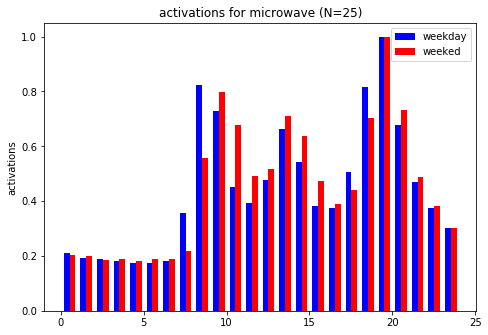
\includegraphics[width=0.9\textwidth]{../Figures/microwave_norm_n25.png}
	\label{fig:UniNormMicrowave}
\end{figure}

One such example can be seen in figure \ref{fig:UniNormMicrowave}. The histogram shows normalized daily 
activation for microwaves. It consists of data from 25 homes from 4 different
datasets. 

The thesis is constructed from three parts, and each answers our following questions accordingly:
\begin{itemize}
	\item How do we efficiently present big data to humans and machines?
	\item How is this presented data connected in a higher dimension?
	\item Can we use one of the profiles to build something useful? 
\end{itemize}

The proposed goal will be achieved by answering these three questions. 
